\documentclass[11pt]{article}

\usepackage[margin=1in]{geometry}
\usepackage{xcolor}
\usepackage{graphicx}
\usepackage{booktabs}
\usepackage{amsmath}
\usepackage{enumitem}
\usepackage[hidelinks]{hyperref}

\newcommand{\file}[1]{\texttt{\detokenize{#1}}}
\newcommand{\code}[1]{\texttt{\detokenize{#1}}}

\newsavebox{\gpbox}
\newenvironment{caveat}[1]{%
  \begin{lrbox}{\gpbox}\begin{minipage}{0.94\linewidth}%
  \textbf{\textcolor{red!55!black}{#1}}\par\smallskip\small}%
 {\end{minipage}\end{lrbox}%
  \begin{center}\setlength{\fboxrule}{0.7pt}%
  \fcolorbox{red!55!black}{red!4}{\usebox{\gpbox}}\end{center}}
\newenvironment{good}[1]{%
  \begin{lrbox}{\gpbox}\begin{minipage}{0.94\linewidth}%
  \textbf{\textcolor{green!35!black}{#1}}\par\smallskip\small}%
 {\end{minipage}\end{lrbox}%
  \begin{center}\setlength{\fboxrule}{0.7pt}%
  \fcolorbox{green!35!black}{green!5}{\usebox{\gpbox}}\end{center}}

\title{\vspace{-1.5em}GCI on Loch --- preliminary results\\[0.3em]
\large A 36-window titration of a CRY1/KL101 hydration site}
\author{}
\date{}

\begin{document}
\maketitle
\vspace{-2.5em}

\section*{Summary}

A full 36-window Grand Canonical Integration titration was run end to end on the Loch
implementation. Every window completed and passed its checkpoint. The titration curve has
the expected sigmoidal shape, the free energy has a well-defined minimum, and the optimal
occupancy agrees with the independently computed equilibrium occupancy.

\textbf{These numbers are not yet publishable.} The sweep ran on the short development
schedule --- 4\,000 GCMC attempts per window against a production 250\,000 --- so the curve
is noisy and required a monotonic fit before it could be integrated. The purpose here is to
show the method and the code path work, not to report a free energy.

\section{What was run}

\begin{center}\small
\begin{tabular}{@{}l l@{}}
\toprule
System & CRY1/KL101, equilibrated through $\mu$VT1 $\to$ NPT $\to$ $\mu$VT2 \\
Site & a pocket water, 2.75 \AA{} from the ligand, 3.09 \AA{} from protein \\
Sphere & $r = 4$ \AA{} at $(48.331,\ 57.025,\ 56.001)$; 27 ghost waters \\
Ladder & 36 values of $B$ from $-30$ to $-4$, finely spaced through the transition \\
Per window & 10 cycles $\times$ (400 GCMC attempts $+$ 200 MD steps) = 4\,000 attempts, 4 ps \\
\midrule
\textbf{Production would be} & \textbf{625 cycles $\times$ (400 $+$ 4\,000) = 250\,000 attempts, 5 ns} \\
\bottomrule
\end{tabular}
\end{center}

All 36 windows completed, and all 36 checkpoints re-validated (every output re-hashed) when
the analysis read them.

\section{The titration curve}

\begin{center}
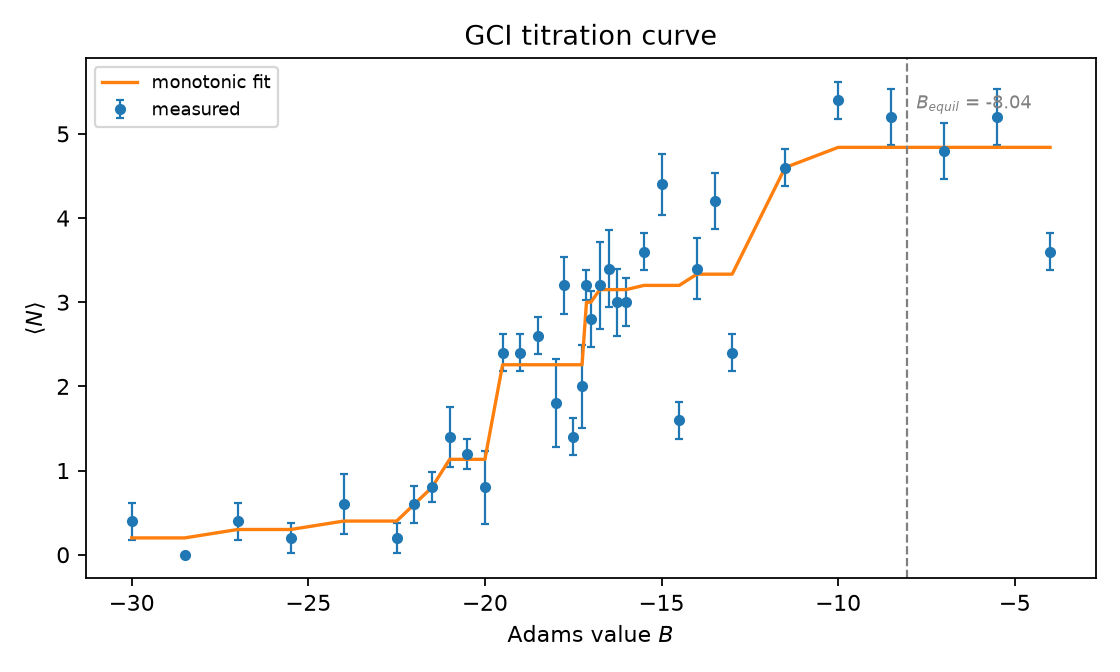
\includegraphics[width=0.93\linewidth]{figures/CRY1KL101_titration_curve.png}
\end{center}

Occupancy rises from zero at $B = -30$ to a plateau of $\sim$5 waters above $B \approx -10$,
with the transition between roughly $B = -21$ and $B = -13$. That is the shape a titration
must have, and it is not built in anywhere: each point is an independent simulation that only
knows its own chemical potential.

Two features are worth pointing at:

\begin{itemize}[nosep,leftmargin=1.4em]
\item \textbf{The low-$B$ tail reaches zero and stays there.} This matters mechanically, not
just aesthetically: it is what sets the lower limit of the integral.
\item \textbf{$B_{\text{equil}} = -8.04$ falls in the plateau} (dashed line). The region is
predicted to be hydrated at equilibrium with bulk water, which is what one expects of a site
that was chosen because it contained a water.
\end{itemize}

The error bars are the spread of the last five checkpoints. They are large relative to the
differences between neighbouring windows, which is the direct cause of the problem in \S4.

\section{The free energy}

Integrating the curve by Ross \emph{et al.} (2015) eq.~19,
\[
\Delta F_{\text{bind}}(N) = k_BT\Big[N B_N - \ln N! - \textstyle\int_{-\infty}^{B_N}\langle N(B)\rangle\,dB\Big] - N\mu'_{\text{hyd}},
\]

\begin{center}
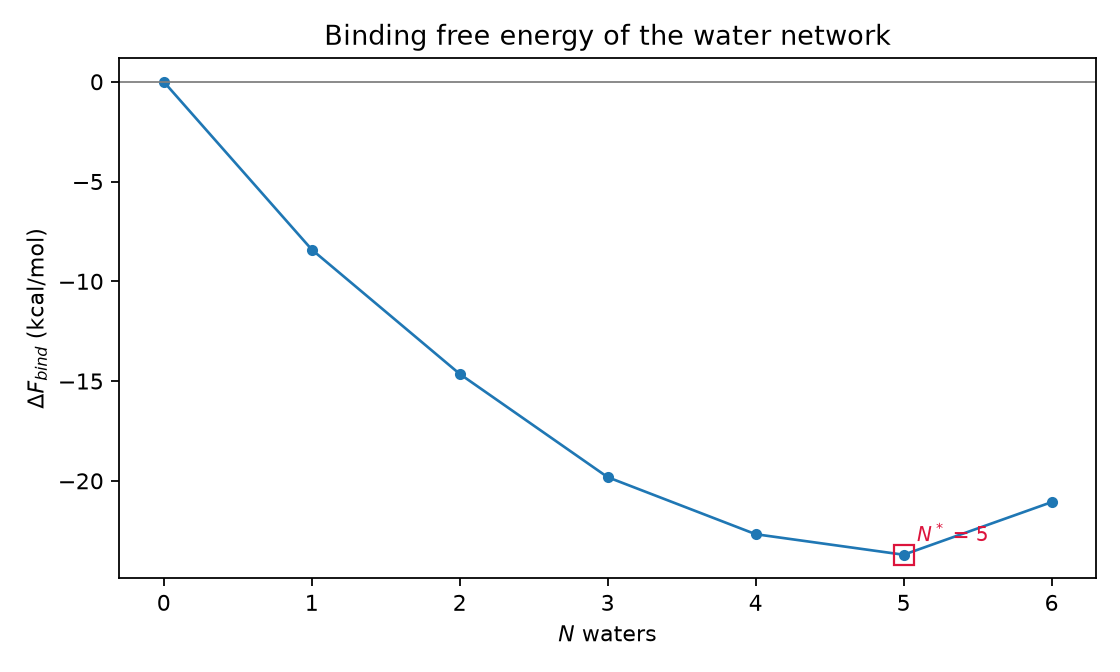
\includegraphics[width=0.93\linewidth]{figures/CRY1KL101_gci_free_energy.png}
\end{center}

\begin{center}\small
\begin{tabular}{@{}r r l@{}}
\toprule
$N$ & $\Delta F_{\text{bind}}$ (kcal/mol) & \\
\midrule
0 & $0.000$ & (by convention) \\
1 & $-8.409$ & \\
2 & $-14.643$ & \\
3 & $-19.818$ & \\
4 & $-22.675$ & \\
\textbf{5} & $\mathbf{-23.705}$ & $\leftarrow N^{*}$, extrapolated \\
6 & $-21.068$ & extrapolated \\
\bottomrule
\end{tabular}
\end{center}

The curve turns over cleanly: each added water is worth progressively less until the fifth,
after which the network is destabilised. That turnover is the whole point of GCI, and it is
present.

\begin{good}{Two internal consistency checks pass}
\begin{itemize}[nosep,leftmargin=1.2em]
\item $\langle N\rangle$ at $B_{\text{equil}}$ is \textbf{4.84}, and the free-energy minimum
is at $N^{*} = \mathbf{5}$. These are computed by different routes --- one interpolates the
curve, the other integrates it --- so their agreement is a real check on the machinery.
\item The ghost reservoir never fell below 26 of 27 in any window, so the high-$B$ tail was
not clipped by the buffer. This was a live concern: the original study's larger sphere had a
buffer roughly equal to its own occupancy.
\end{itemize}
\end{good}

For orientation only: this gives $-4.74$ kcal/mol per water, against $-4.70$ from the
published CRY1/AN139 Sphere 2 result ($N^{*}=2$, $\Delta F = -9.397$). The agreement is
closer than the data deserves --- different ligand, different site, under-converged sampling
--- so treat it as "the right order of magnitude", not as validation.

\section{What is not yet right}

\begin{caveat}{The curve is not monotonic, and had to be fitted}
$\langle N\rangle$ must be non-decreasing in $B$ for the inverse interpolation that gives
$B_N$ to mean anything. The measured curve has \textbf{14 inversions} --- e.g.\
$\langle N\rangle(-15.0) = 4.4$ but $\langle N\rangle(-14.5) = 1.6$.

These are noise, not physics. Each window is 4\,000 attempts and 4 ps of MD, and the tail
average is five checkpoints, so the per-point spread (0.4--1.2 waters) is comparable to the
spacing between windows.

\file{gci_analyse.py} \textbf{refuses by default} on such input and names the offending
windows. The numbers above come from the opt-in isotonic (monotone least-squares) fit, and
are labelled preliminary throughout.
\end{caveat}

Two further consequences of the short schedule:

\begin{itemize}[nosep,leftmargin=1.4em]
\item $N^{*} = 5$ sits at the edge of the sampled range, so $B_{N}$ for $N \ge 5$ is
\emph{extrapolated}. The reported minimum is therefore the least reliable point on the curve.
\item The high-$B$ end does not cleanly plateau in the raw data (it wanders between 3.6 and
5.4), which is what pushes the integral onto that extrapolation.
\end{itemize}

\section{Conclusion and next step}

The implementation works. A site is anchored by a massless dummy atom, each window samples at
a verified Adams value, occupancy is recorded as a machine-readable observable, 36 windows
integrate into a free-energy curve with a physically sensible minimum, and two independent
consistency checks agree. Nothing in the chain from equilibrated structure to
$\Delta F_{\text{bind}}$ is missing.

What remains is sampling. Re-running with \code{SMOKE=0} gives 62$\times$ more GCMC attempts
and 1\,000$\times$ more MD per window, which is what the monotonicity and the high-$B$
plateau require. At that point the isotonic fit should become unnecessary --- and the right
way to report the result is to run the analysis in its default mode and let it either accept
the curve or refuse it.

\vspace{0.5em}
\noindent\small\textit{Artifacts:} \file{gci_runs/} (36 windows, each with its own titration
CSV, metadata JSON and checkpoint); \file{figures/} (pooled curve, free-energy table,
figures, summary JSON, checkpoint).

\end{document}
